\documentclass{beamer}
%\title{nazwa prezentacji}
\author{Klaudia Rutkowska}
\date{\today}
\institute{UWM}
\usepackage{amsfonts}
\usepackage{graphicx}
\usepackage[MeX]{polski}
\begin{document}
\frame{\titlepage}
%\begin{frame}
%\frametitle{Spis tre�ci}
%\tableofcontents
%\end{frame}

%http://wmii.uwm.edu.pl/~denisjuk/uwm/ni/wyklady/06-projects.pdf
%http://wmii.uwm.edu.pl/~denisjuk/uwm/ni/

%\begin{table}  szablon przyk�adowej tabeli
%\begin{tabular}{lccc}
%\hline
%\textbf{stanowisko}&\textbf{osoba}&\textbf{od}&\textbf{do}\\
%\hline
%premier&Ben Chilfley&1 listopada 1946 & 19 grudnia 1949\\
%minister skarbu&Ben Chifley&1 listopada 1946&19 grudnia 1949\\
%minister obrony&John Dedman&1 listopada 1946&19 grudnia 1949\\
%minister si� powietrznych&Arthur Drakeford&1 listopada 1946&19 grudnia 1949\\
%minister imigracji&Arthur Calwell&1 listopada 1946&19 grudnia 1949\\
%minister zaopatrzenia rozwoju&John Armstrong&6 kwietnia 1948&19 grudnia 1949\\
%\hline
%\end{tabular}
%\caption{Sklad}
%\end{table}

%\begin{frame}{Archeologia podwodna -cd.} jest to szablon dodawania zdjecia
%\begin{center}
%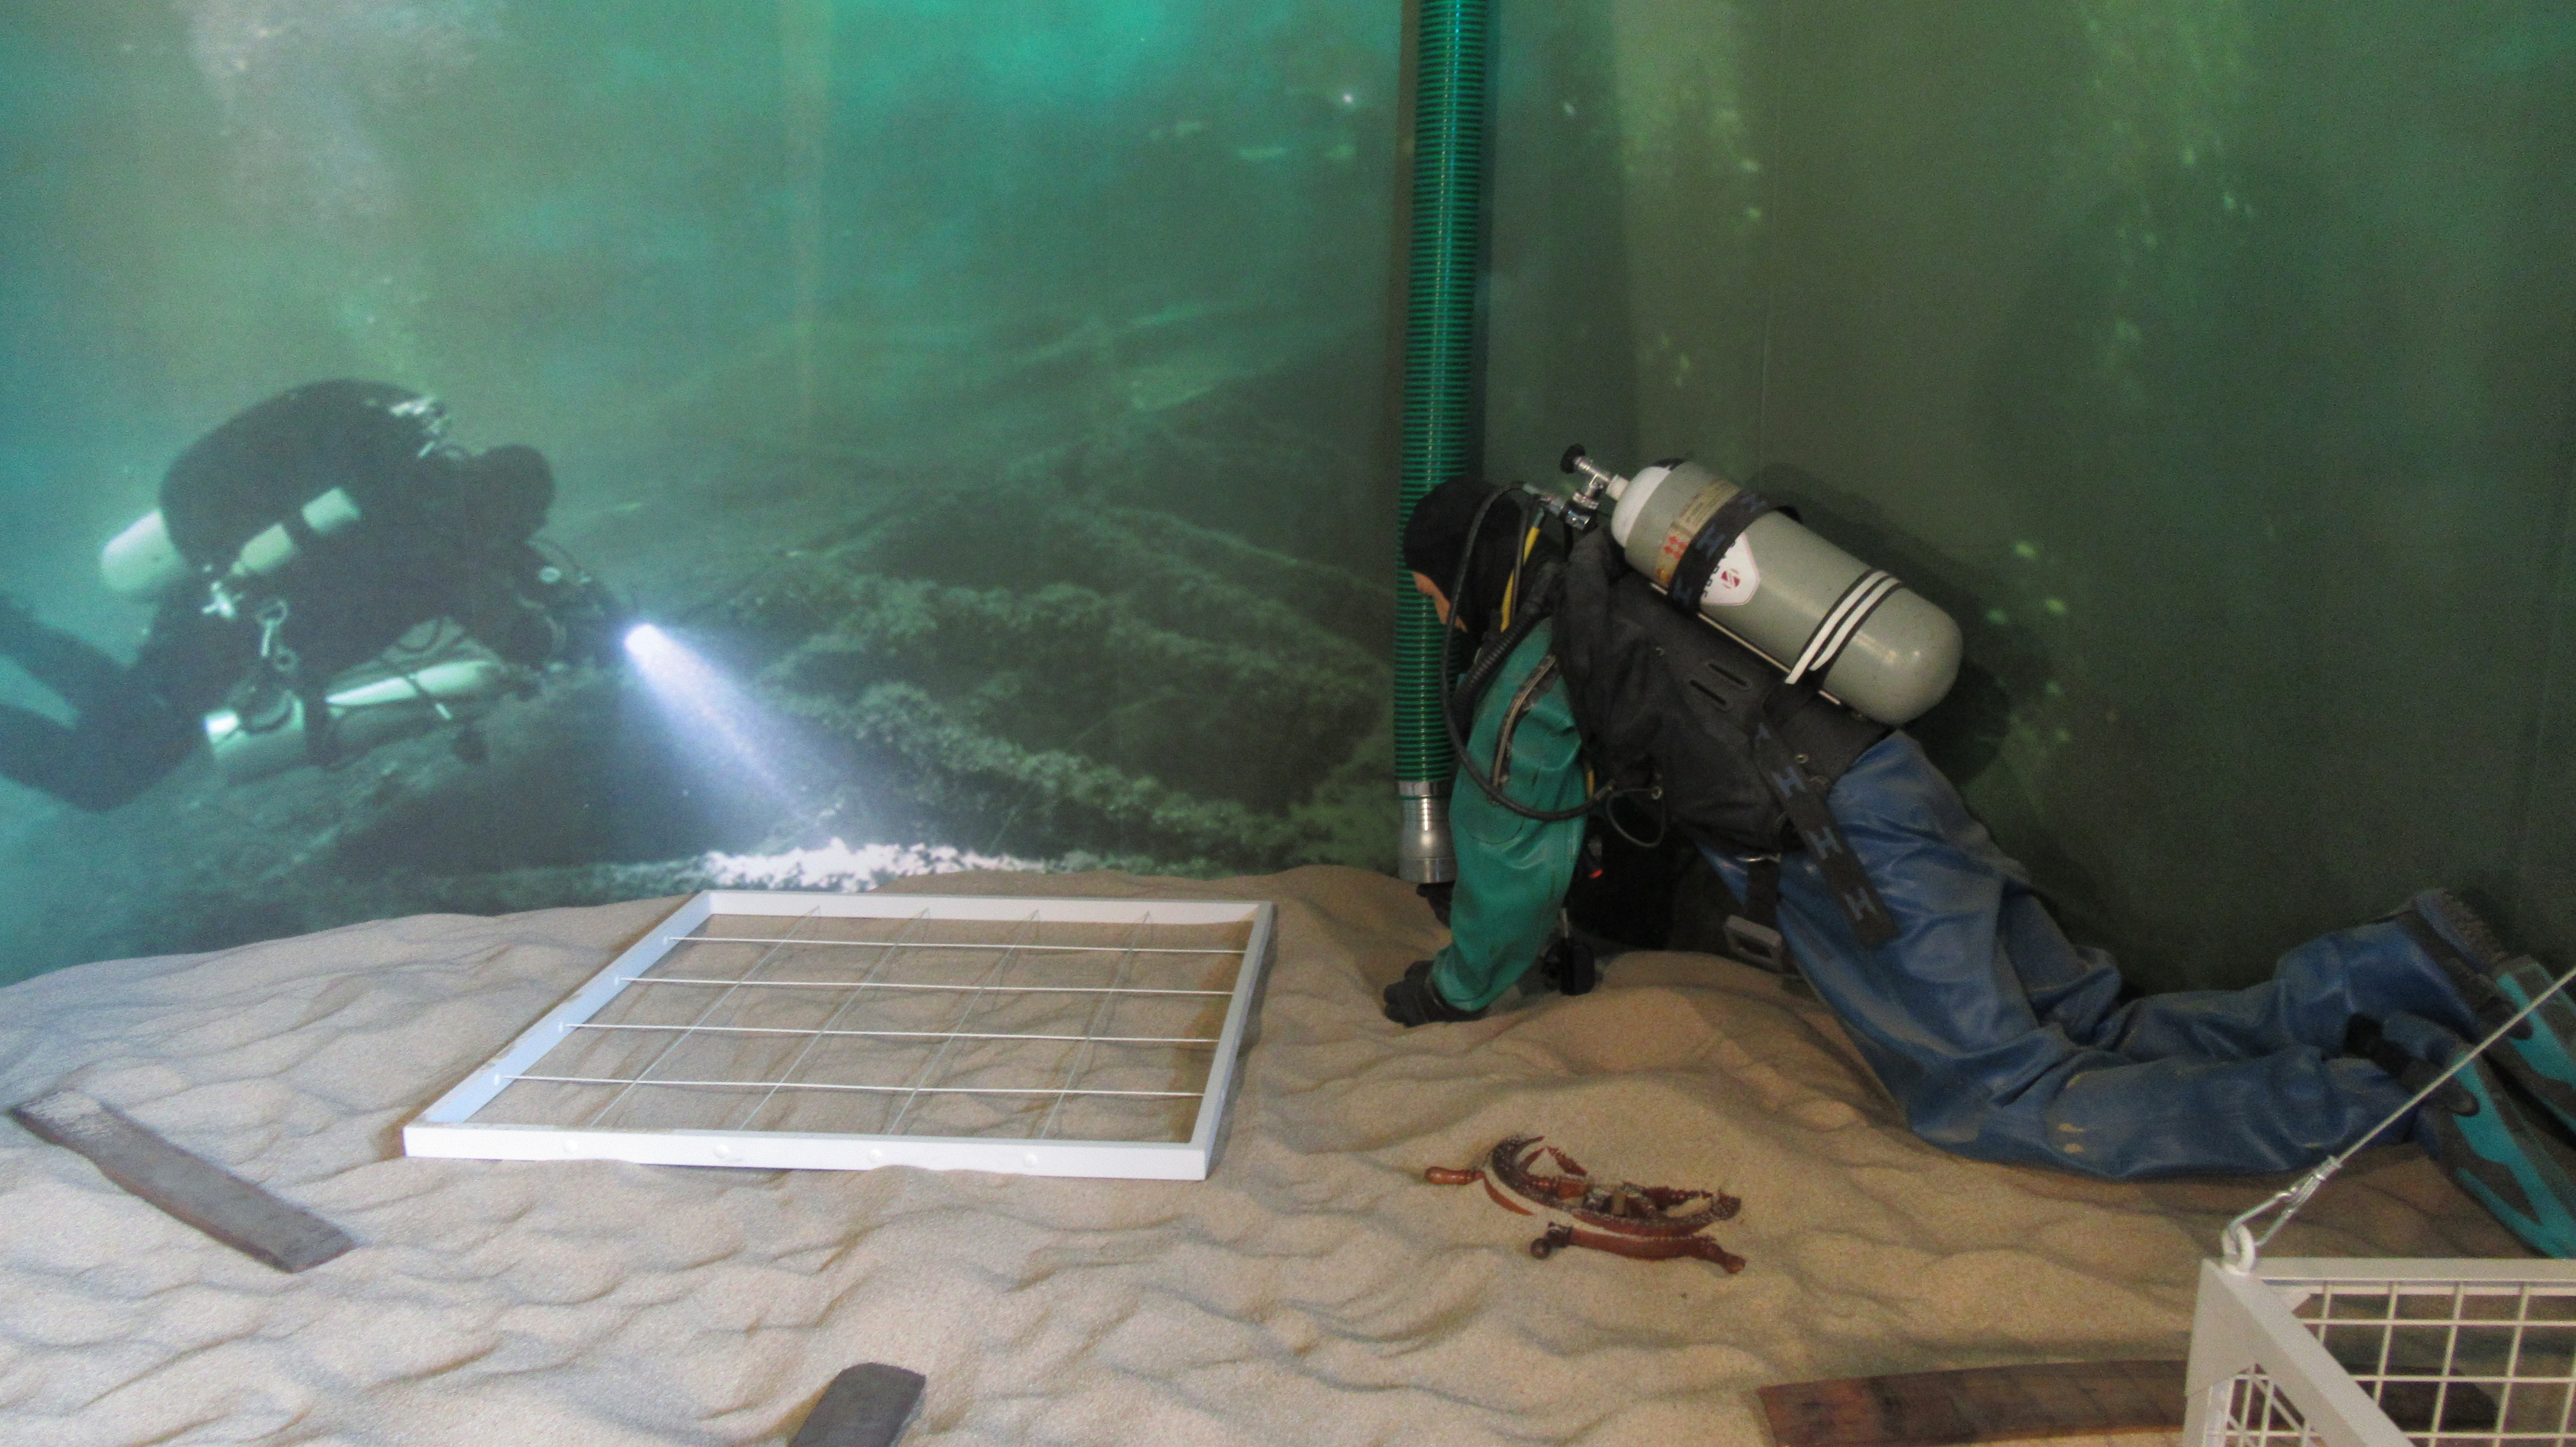
\includegraphics[width=8cm]{mumin.jpg}
%\label{mumin.jpg}
%\end{center}
%\end{frame}

%\begin{frame}{tytul slajdu}  jest to szablon slajdu
%\section{tutaj jakby odno�nik z boku}
%tekst
%\end{frame}

\end{document}
